\let\negmedspace\undefined
\let\negthickspace\undefined
\documentclass[journal]{IEEEtran}
\usepackage[a5paper, margin=10mm, onecolumn]{geometry}
%\usepackage{lmodern} % Ensure lmodern is loaded for pdflatex
\usepackage{tfrupee} % Include tfrupee package

\setlength{\headheight}{1cm} % Set the height of the header box
\setlength{\headsep}{0mm}     % Set the distance between the header box and the top of the text

\usepackage{gvv-book}
\usepackage{gvv}
\usepackage{cite}
\usepackage{amsmath,amssymb,amsfonts,amsthm}
\usepackage{algorithmic}
\usepackage{graphicx}
\usepackage{textcomp}
\usepackage{xcolor}
\usepackage{txfonts}
\usepackage{listings}
\usepackage{enumitem}
\usepackage{mathtools}
\usepackage{gensymb}
\usepackage{comment}
\usepackage[breaklinks=true]{hyperref}
\usepackage{tkz-euclide} 
\usepackage{listings}
% \usepackage{gvv}                                        
\def\inputGnumericTable{}                                 
\usepackage[latin1]{inputenc}                                
\usepackage{color}                                            
\usepackage{array}                                            
\usepackage{longtable}                                       
\usepackage{calc}                                             
\usepackage{multirow}                                         
\usepackage{hhline}                                           
\usepackage{ifthen}                                           
\usepackage{lscape}
\usepackage{circuitikz}
\tikzstyle{block} = [rectangle, draw, fill=blue!20, 
    text width=4em, text centered, rounded corners, minimum height=3em]
\tikzstyle{sum} = [draw, fill=blue!10, circle, minimum size=1cm, node distance=1.5cm]
\tikzstyle{input} = [coordinate]
\tikzstyle{output} = [coordinate]


\begin{document}

\bibliographystyle{IEEEtran}
\vspace{3cm}

\title{4.4.27}
\author{AI25BTECH110031 \\ Shivam Sawarkar}
 \maketitle
% \newpage
% \bigskip
{\let\newpage\relax\maketitle}

\renewcommand{\thefigure}{\theenumi}
\renewcommand{\thetable}{\theenumi}
\setlength{\intextsep}{10pt} % Space between text and floats


\numberwithin{equation}{enumi}
\numberwithin{figure}{enumi}
\renewcommand{\thetable}{\theenumi}

\textbf{Question(4.4.27)} Find the value of $x$ such that the points $A (3, 2, 1) , B (4, x, 5) , C (4, 2, -2)$ and $D (6, 5, -1)$ are coplanar. \\ 
\textbf{Solution:} \\ 
Let the plane (not passing through the origin) be given by
\begin{align}
\vec{n}^\top\vec{x}=1,\qquad 
\vec{n}=\myvec{n_1 \\ n_2 \\ n_3}
\end{align}
Since the points 
\begin{align}
    \vec{A}=\myvec{3 \\ 2 \\ 1} \quad
    \vec{B}=\myvec{4 \\ 2 \\ -2} \quad
    \vec{C}=\myvec{6 \\ 5 \\ -1}
\end{align}
lie on the plane, they satisfy 
\begin{align}
    \vec{n}^\top\vec{A}=1 \\ 
    \vec{n}^\top\vec{B}=1 \\ 
    \vec{n}^\top\vec{C}=1
\end{align}

\begin{align}
\myvec{
3 & 2 & 1\\ 
4 & 2 & -2\\ 
6 & 5 & -1
}
\myvec{n_1\\ n_2\\ n_3}
=
\myvec{1 \\ 1 \\ 1}.
\end{align}

Thus
\begin{align}
n_1=\frac{9}{16},\qquad n_2=-\frac{7}{16},\qquad n_3=\frac{3}{16}.
\end{align}

Now require B to lie on the same plane:
\begin{align}
\vec{n}^\top\vec{B}=1 \\ 
\myvec{\frac{9}{16} & \frac{-7}{16} & \frac{3}{16}}\myvec{4 \\ x \\ 5}=1
\end{align}
\begin{align}
\frac{36}{16} - \frac{7}{16}x + \frac{15}{16} = 1 \\ 
51-7x=16 
\end{align}

\begin{align}
\boxed{x=5}
\end{align}

\begin{figure}[H]
    \centering
    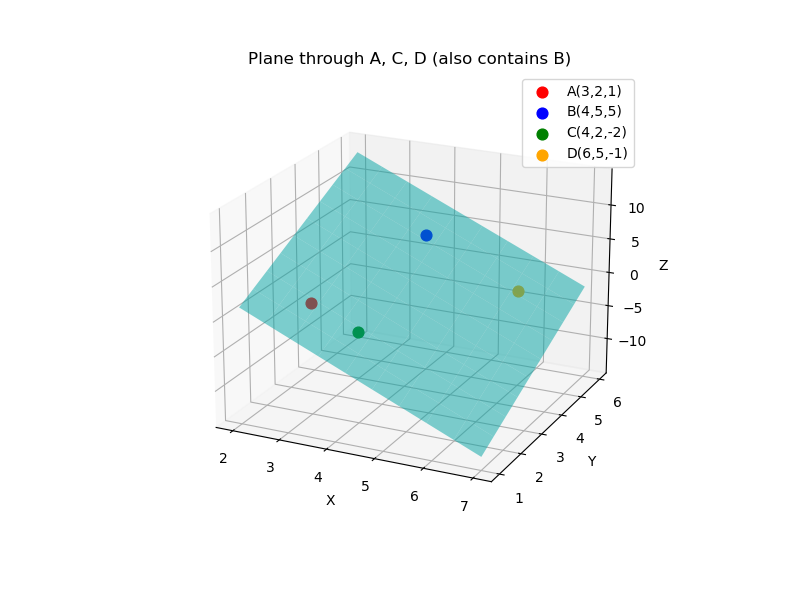
\includegraphics[width=1\linewidth]{figs/plot7.png}
    \caption{}
    \label{fig:placeholder}
\end{figure}






\end{document}